In the early 1990's, Ullas Karanth (Fig. \ref{fig.karanth})
asked my advice on estimating tiger
density from camera-trap data. Historic uses of camera traps had been
restricted to wildlife photography and the documentation of species
presence. Ullas had the innovative idea to extend these uses to
inference about tiger population size, density and even survival and
movement by exploiting the individual markings of tigers.  I had
worked on development and application of capture-recapture models, so
we began a collaboration that focused on population inferences based
on detection histories of marked tigers. Early on in this work, we had
to consider how to deal with two problems associated with the spatial
distributions of both animals and traps.


\begin{figure}[h!]
\centering
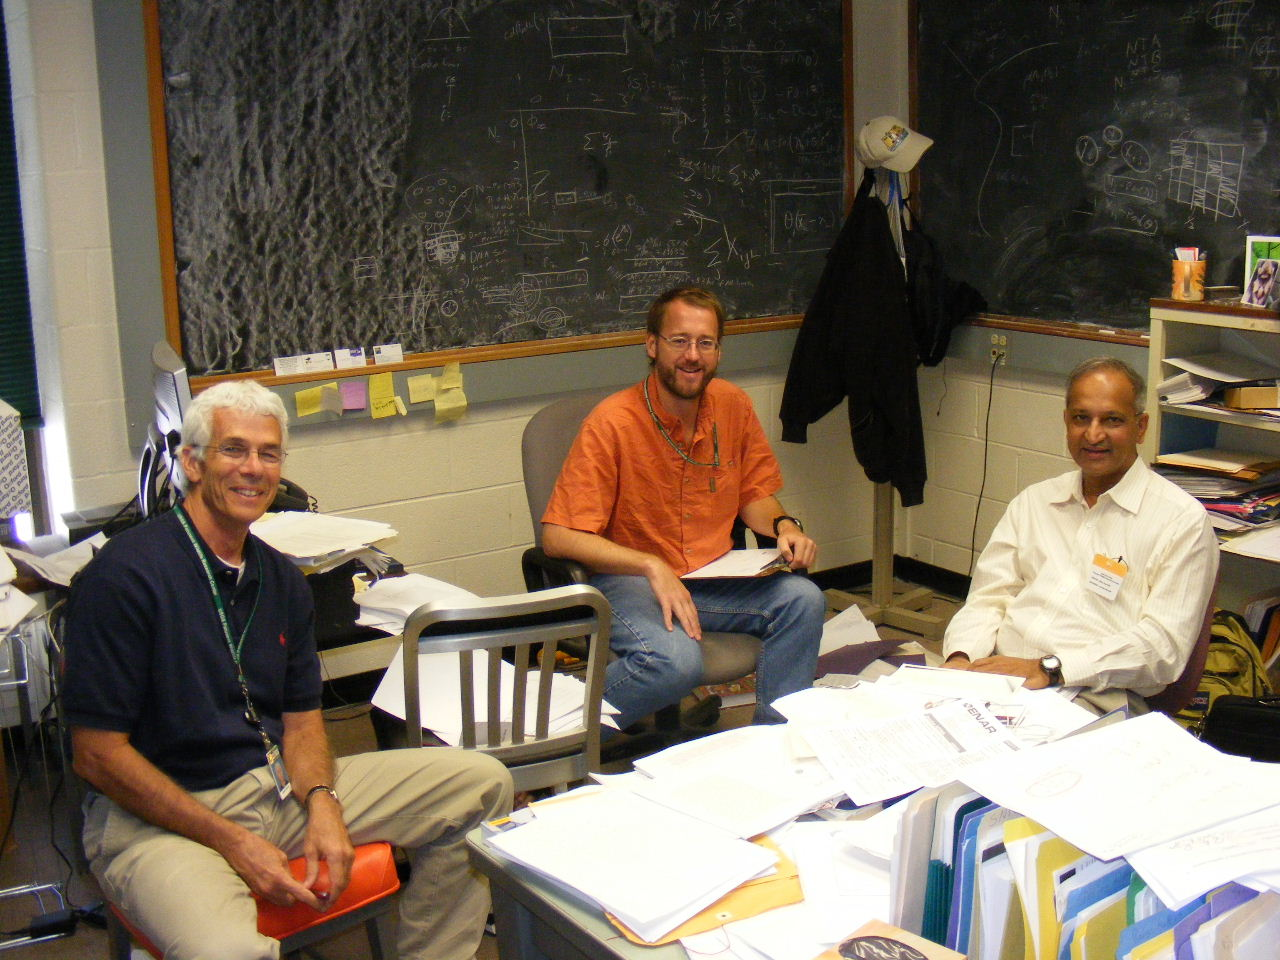
\includegraphics[height=3.5in]{Ch0-Foreword/Nichols_etal.jpg}
\caption{
Jim Nichols (left) discussing capture-recapture with K. Ullas Karanth
and Andy Royle at Patuxent Wildlife Research Center, 
Oct. 15, 2007. 
}
\label{fig.karanth}
\end{figure}

The first problem was that of heterogeneous capture probabilities
among animals resulting from the positions of their ranges relative to
trap locations. Animals with ranges centered in the middle of a
trapping array are much more likely to encounter traps and be captured
than animals with range centers just outside the trapping array. Ad
hoc abundance estimators were available to deal with such
heterogeneity, and we resolved to rely primarily on such estimators
for our work.  


Ullas was more interested in tiger density (defined
loosely as animals per unit area) than in abundance, and the second
problem resulted from our need to translate abundance estimates into
estimates of density.  This translation required inference about the
total area sampled, that is the area containing animals exposed to
sampling efforts. In the case of fixed sampling devices such as traps
and cameras, the area sampled is certainly greater than the area
covered by the devices themselves (e.g., as defined by the area of the
convex hull around the array of devices), but how do we estimate this
area?  This problem had been recognized and considered since the
1930's, and ad hoc approaches to solving it included nested grids,
assessment lines, trapping webs and use of movement information from
either animal recaptures or radiotelemetry data. We selected an
approach using distances between captures of animals.  

We thus
recognized these two problems caused by spatial distribution of
animals and traps, and we selected approaches to deal with them as
best we could. We were well aware of the ad hoc nature of our
pragmatic solutions. In particular, we viewed the use of movement
information based on recaptures to translate our abundance estimates
into density estimates as the weak link in our approach to inference
about density. 

 In the early 2000's, Murray Efford developed a novel
approach to inference about animal density based on capture-recapture
data. The manuscript on this work was rejected initially by a top
ecological journal without review (an interesting comment on the
response of our peer review system to innovation), but was published
in Oikos in 2004. The approach was anchored in a conceptual model of
the trapping process in which an animal's probability of being
captured in any particular trap was a decreasing function of the
distance between the animal's home range center and the trap. This
assumed relationship was very similar to the key relationship on which
distance sampling methods are based. Efford viewed the distribution of
animal range centers as being governed by a spatial point process, and
the target of estimation was the intensity of this process, equivalent
to animal density in the study area. \citet{efford:2004}
initially used an
ad hoc approach to inference based on inverse prediction. He later
teamed with David Borchers to develop a formal likelihood approach to
estimation (Borchers and Efford 2008 and subsequent papers).  


At about the same time that Efford was formalizing his approach, yet
independently of that work, Andy Royle developed a similar approach
for the related problem of density estimation based on locations of
captures of animals obtained during active searches of prescribed
areas (as opposed to captures in traps with fixed locations). Andy
approached the inference problem using explicit hierarchical models
with both a process component (the spatial distribution of animal
range centers and a probability distribution reflecting movement about
those centers) and an observation component (non-zero capture
probability for locations within the surveyed area and 0 outside this
area). He used the data augmentation approach that he had just
developed \citep{royle_etal:2007} to deal with animals in the
population that are never captured, and he implemented the model using
Markov chain Monte Carlo sampling \citep{royle_young:2008}.  Ullas and
I asked Andy for help (Fig. \ref{fig.karanth}) with inference about
tiger densities, and he extended his approach to deal with fixed trap
locations by modeling detection probability as a function of the
distance between range center and trap, thus solving our two
fundamental problems emanating from spatial distributions of animals
and traps \citep{royle_etal:2009japple, royle_etal:2009ecol}.

The preceding narrative about the solution of two inference problems
faced by Ullas Karanth and me was presented to motivate interest in
the models that are the subject of {\it Spatial
  Capture-Recapture}. SCR models provide a formal solution to the
problem of heterogeneous capture probabilities associated with
locations of animal ranges relative to trap locations. They also
provide a formal and direct (as opposed to ad hoc and indirect) means
of estimating density, naturally defined for SCR models as number of
range centers per unit area.  This motivation is perhaps adequate, but
it is certainly incomplete. As noted in this book's introduction, SCR
models should not be viewed simply as extensions of standard
capture-recapture models designed to solve specific spatial
problems. Rather, SCR models represent a much more profound
development, dealing explicitly with ecological processes associated
with animal locations and movement as well as with the spatial aspects
of sampling natural populations. They provide improvements over
standard capture-recapture models in our abilities to address
questions about demographic state variables (density, abundance) and
processes (survival, recruitment), and they provide new possibilities
for addressing questions about spatial organization and space use by
animals.

As the promise of SCR models has become recognized, work on them has
proliferated over the last five years, with substantive new
developments led in part by the authors of this book, Andy Royle,
Richard Chandler, Rahel Sollman and Beth Gardner. Because of this
explosive development, it is no longer possible to consult one or two
key papers in order learn about SCR. Royle and colleagues recognized
the need for a synthetic treatment to integrate this work and place it
within a common framework. They wrote {\it Spatial Capture-Recapture}
in order to fill this need.

The history of methodological development in quantitative ecology
contains numerous examples of synthetic books and monographs that have
been extremely influential in advancing the use of improved inference
procedures. {\it Spatial Capture-Recapture} will become a part of this
history, serving as a catalyst for use and further development of SCR
methods. The writing style is geared to a biological readership such
that this book will provide a single source for biologists interested
in learning about SCR models. The statistical development is
sufficiently rigorous and complete that this synthesis of existing
work should serve as a springboard for statisticians interested in
extensions and new developments. I believe that Spatial
Capture-Recapture will be an extremely important book.

{\it Spatial Capture-Recapture} is organized around four major
sections (plus appendices). The first, ``Background and Concepts'',
provides motivation for SCRs and a history of relevant concepts and
modeling. Two chapters are devoted to statistical background, one
including material introducing random variables, common probability
distributions, and hierarchical models. The second chapter on
statistical background develops the concept of SCRs as generalized
linear mixed models, with some emphasis on Bayesian inference methods
for such models. Also included in this section is a chapter on
standard (non-spatial) capture-recapture models for closed
populations. This chapter helps motivate SCRs and introduces the idea
of data augmentation as an approach to dealing with zero-inflated
models for inference about abundance. The authors develop a primitive
SCR model in this chapter by noting that location data for captured
animals can be viewed as individual covariates.


The second major section, ``Basic SCR Models'',
begins with a complete development of SCRs as hierarchical models with
observation and spatial point process components. Included is a clear
discussion of space use by animals, important because any model of the
detection process implies a model for space use. A chapter is devoted
to likelihood analysis of SCR models including both model development
and an introduction to software available for fitting models. Another
chapter is devoted to various approaches to modeling variation in
encounter probability. A variety of basic models is introduced, as
well as approaches to modeling covariates associated with traps, time,
individual capture history, and individual animals (e.g., sex, body
mass, random effects models as well). The chapter on model selection
and assessment does not provide an omnibus, one-size-fits-all
statistic. Rather, it describes useful approaches including AIC for
likelihood analyses and both DIC and the \citet{kuo_mallick:1998}
indicator variable approach for Bayesian analyses. For assessing model
adequacy, they use the Bayesian p-value approach \citep{gelman_etal:1996}
applied to different components of model fit. Another chapter is
devoted to the encounter process which requires attention to the
nature of the detection device (e.g., can an animal be caught only
once or multiple times during an occasion, do traps permit catches of
multiple or only single individuals, can an individual be detected
multiple times by the same device) and the kinds of data produced by
these devices. The final chapter in this section deals with the
important topic of study design. A fundamental design trade-off
involves the competing needs to capture a good number of animals
(sample size) and to attain a reasonably high average capture
probability, and the authors emphasize the need for designs that
represent a good compromise rather than those that emphasize one
component to the exclusion of the other. General recommendations about
trap spacing and clustering, and use of ancillary data (telemetry) are
discussed as well. The material in this section is extremely important
in conveying the basic principles underlying SCR modeling and, as
such, will be the section of primary interest to many readers.  

The
next section, ``Advanced SCR Models'', will be of great interest to
ecologists, not just because of the advanced model structures
presented, but because of the ecological questions that become
accessible using these methods. For example, the authors show how
spatial variation in density can be modeled as a function of spatial
covariates associated with all locations in the state
space. Similarly, the authors relax the assumption of basic SCR models
that encounter probability is a function of Euclidean distance between
range center and trap, and focus instead on the ``least cost path''
between the range center and trap. The least cost path concept is
modeled by including resistance parameters related to habitat
covariates, and is relevant to the ecological concepts of connectivity
and variable space use. The authors note ecological interest in
resource selection functions, which focus on animal use of space as a
function of specific resource or habitat covariates and which are
typically informed by radiotelemetry data. They present a framework
for development of joint models that combine SCR and resource
selection function telemetry data. In some situations, sampling is
done via a search encounter process rather than using detection
devices with fixed locations, and SCR models are extended to deal with
these. Models are developed for combining data from sampling at
multiple sites or across multiple occasions. The extension of the SCR
framework to models for open populations permits inference about the
processes of survival, recruitment and movement. Inference about
time-specific changes in space use is also directly accessible using
this approach, and I anticipate a great many advances in the
development and application of open population SCR models. 


 The final
section, ``Super-Advanced SCR Models'', includes a technical chapter on
development of MCMC samplers for the primary purpose of providing
increased flexibility in SCR modeling. A chapter of huge potential
importance introduces SCR models for unmarked populations, relying on
the spatial correlation structure of resulting count data to draw
inferences about animal distribution and density.  These models will
see widespread use in studies employing remote detection devices
(camera traps, acoustic detectors) to sample animals that do not
happen to have individually recognizable visual patterns or acoustic
signatures. In many sampling situations, some animals will be
individually identifiable and many will not, and the authors develop
mark-resight models to combine detection data from these two classes
of animals.  The final chapter provides a glimpse of the future by
pointing to a sample of neat developments that should be possible
using the conceptual framework provided by SCR models.  

I very much
like the writing style of the authors and found the book relatively
easy to read (there were exceptions), with clear presentations of
important ideas. Most models are illustrated nicely with actual
examples and corresponding sample computer code (frequently WinBUGS).


In summary, I repeat my claim that {\it Spatial Capture-Recapture} is an
extremely important and useful book. A thorough read of the section on
basic SCR models provides a good understanding of exactly how these
models are constructed and how they ``work'' in terms of underlying
rationale. The two sections on advanced SCR models present a thorough
account of the current state of the art written by those who have
largely defined this state. As an ecologist, I found myself thinking
of one potential application of these models after another. These
methods will free ecologists to begin to think more clearly about
interesting questions concerning the statics and dynamics of space use
by animals. The ability to draw inferences about distribution and
density of animals based on counts of unmarked individuals using
remote detection devices has the potential to revolutionize
conservation monitoring programs.  

So does {\it Spatial Capture-Recapture}
solve the inference problems encountered by Ullas Karanth and me two
decades ago? You bet. But it does so much more than that. Andy,
Richard, Rahel and Beth, thanks for an exceptional contribution.

\vspace{.3in}

{\flushleft 
James D. Nichols}  \\ 
{\flushleft Patuxent Wildlife Research Center }  \\
{\flushleft March 14, 2013 }
